\newpage
\section*{Appendix A\quad The calculus, for readers who want it}
\addcontentsline{toc}{section}{A The calculus}
\startchapter{A}
\providecommand{\fitR}[1]{\leavevmode\setbox0\hbox{#1}\ifdim\wd0>\linewidth\resizebox{\linewidth}{!}{\box0}\else\box0\fi}

\begin{chaptermap}
Chapter 8 found slopes by probing: step a little left, a little right, compare. This appendix shows how the
slopes are computed exactly, for every knob at once. We start from the slope of a curve (\S A.1), add the one
rule that does all the work, the chain rule (\S A.2), and then apply it to the three places that matter in a
transformer: the loss at the end (\S A.3), attention (\S A.4) and the residual connection (\S A.5). Every
formula here was checked by a script, \texttt{code/appA\_check.py}, against the probing method of Chapter 8.
The largest disagreement anywhere is $\nAppAErrMax$ (a relative error), which is rounding noise.
\end{chaptermap}

\begin{beforeyoustart}
\begin{enumerate}[label=(\arabic*),leftmargin=1.6em]
\item The slope of a straight line is ``rise over run''. A line goes through $(1,2)$ and $(3,8)$. Slope?
\emph{Refresher: $(8-2)/(3-1)=3$.}
\item What is $(a+b)^2$? \emph{Refresher: $a^2+2ab+b^2$.}
\item A matrix of shape $3\times4$ times one of shape $4\times2$ gives what shape? \emph{Refresher: $3\times2$;
the inner sizes must match and disappear (Chapter 3, \S3.4).}
\end{enumerate}
\end{beforeyoustart}

\subsection*{A.1\quad From the slope of a line to the slope of a curve}

\Predict The curve $y=x^2$ is not a straight line, so its steepness changes from place to place. How steep is
it at $x=3$? Guess a number before reading on.

\Picture Zoom in on a curve far enough and it looks like a straight line. The slope of that tiny straight
piece is the slope of the curve at that point.

Let us zoom in on $y=x^2$ at $x=3$, using the rise-over-run of a short step $h$:
\[
\frac{(3+h)^2 - 3^2}{h}\quad\text{gives}\quad \nAppASlopeOne\ (h=1),\qquad \nAppASlopeTenth\ (h=0.1),\qquad
\nAppASlopeThousandth\ (h=0.001).
\]
The numbers settle towards 6. \Exactly Expanding, $\big((3+h)^2-9\big)/h = (6h+h^2)/h = 6+h$, and as the
step $h$ shrinks to nothing this becomes exactly 6. That limit is the \emph{derivative}, written
$\frac{dy}{dx}$. Doing the same at a general $x$ gives $\frac{d}{dx}x^2 = 2x$.

\Why Probing (Chapter 8) is this formula with a small but not-zero $h$. The derivative is what probing would
give with a step too small to measure. It is exact, and it costs nothing extra once you know the formula.

\begin{checkq}
Probing $y=x^2$ at $x=3$ with $h=0.1$ gave 6.1, not 6. Why the extra 0.1?
\begin{options}
\item Rounding error in the computer.
\item The curve bends within the step, and the bend adds $h$ to the rise-over-run.
\item The derivative of $x^2$ is $2x+0.1$.
\end{options}
\end{checkq}

\subsection*{A.2\quad The chain rule: slopes multiply}

\Picture Three gears in a row. If the first turns the second 3 times as fast, and the second turns the third
2 times as fast, the first turns the third $3\times2=6$ times as fast. When one quantity feeds another, the
rates multiply.

\Exactly If $y=f(u)$ and $u=g(x)$, then
\[
\frac{dy}{dx}=\frac{dy}{du}\cdot\frac{du}{dx}.
\]
Example: $y=(3x+1)^2$. Let $u=3x+1$, so $y=u^2$. Then $dy/du=2u$ and $du/dx=3$, so $dy/dx = 2(3x+1)\cdot3$,
which at $x=1$ is $2\cdot4\cdot3 = 24$. Probing with a tiny step gives \nAppAChainNum.

With many knobs, the slope of the loss with respect to each knob is called a \emph{partial derivative},
written $\partial L/\partial w$; the list of all of them is the gradient. \emph{Backpropagation} is the chain
rule applied from the loss backwards, layer by layer: each layer receives ``how much the loss changes when my
output changes'' and passes back ``how much the loss changes when my input changes'', multiplying by its own
local slope. Every intermediate result is computed once and reused, which is why the whole gradient costs
about as much as one extra forward pass.

\Summary{a derivative is the slope of a tiny straight piece of a curve, and the chain rule multiplies local
slopes along any path from a knob to the loss.}

\subsection*{A.3\quad The loss at the end: prediction minus answer, after all}

Let the scores (logits) be $\bm{z}$, the probabilities $\bm{p}=\softmax(\bm{z})$, and the right word be $y$.
The loss is $L=-\ln p_y$. Write it out:
\[
L = -\ln\frac{e^{z_y}}{\sum_j e^{z_j}} = -z_y + \ln\sum_j e^{z_j}.
\]
The slope of the first part with respect to $z_i$ is $-1$ if $i=y$ and 0 otherwise. The slope of the second
part, by the chain rule, is $e^{z_i}/\sum_j e^{z_j} = p_i$. So
\[
\frac{\partial L}{\partial z_i} = p_i - [\,i=y\,] \shape{1\times V},
\]
where $[\,i=y\,]$ is 1 for the right word and 0 otherwise. Here is the twist promised in Chapter 8: the
correction \emph{is} ``prediction minus answer'', one probability at a time, with the answer written as a 1
for the right word and 0 for the rest. For our toy after \tok{waste of time}: the slope on the \tok{Sorry}
score is \nAppAGradSorry\ (negative, so walking downhill raises it) and on the \tok{been} score
\nAppAGradBeen\ (positive, so it is lowered). Checked against probing: relative error $\nAppAErrCE$.
Here are all three vectors for the toy:

\par\medskip\noindent\begin{minipage}{\linewidth}\centering
\fitR{% AUTO-GENERATED by code/figlib.py helpers -- do not edit
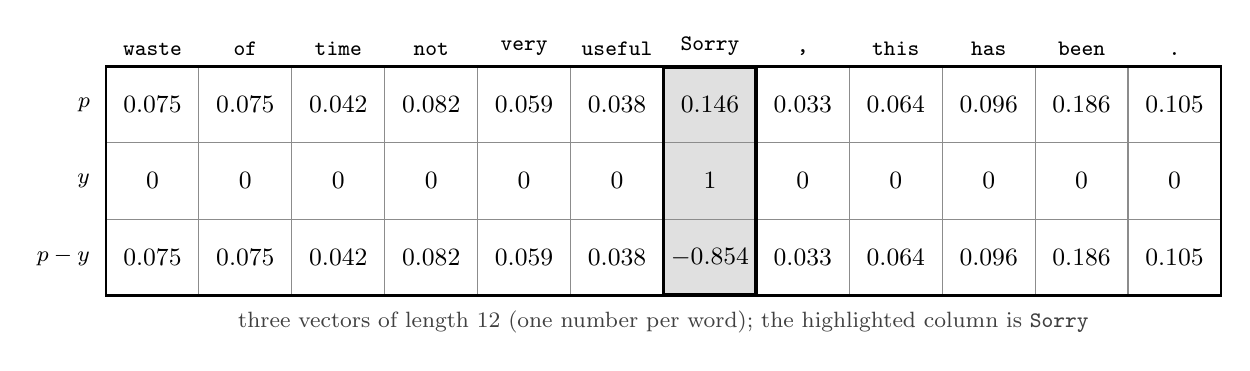
\begin{tikzpicture}
\draw[black!45, fill=white] (0.000,0.000) rectangle (1.180,-0.968);
\node[font=\small, text=black] at (0.590,-0.484) {$0.075$};
\draw[black!45, fill=white] (1.180,0.000) rectangle (2.360,-0.968);
\node[font=\small, text=black] at (1.770,-0.484) {$0.075$};
\draw[black!45, fill=white] (2.360,0.000) rectangle (3.540,-0.968);
\node[font=\small, text=black] at (2.950,-0.484) {$0.042$};
\draw[black!45, fill=white] (3.540,0.000) rectangle (4.720,-0.968);
\node[font=\small, text=black] at (4.130,-0.484) {$0.082$};
\draw[black!45, fill=white] (4.720,0.000) rectangle (5.900,-0.968);
\node[font=\small, text=black] at (5.310,-0.484) {$0.059$};
\draw[black!45, fill=white] (5.900,0.000) rectangle (7.080,-0.968);
\node[font=\small, text=black] at (6.490,-0.484) {$0.038$};
\draw[black!45, fill=black!12] (7.080,0.000) rectangle (8.260,-0.968);
\node[font=\small, text=black] at (7.670,-0.484) {$0.146$};
\draw[black!45, fill=white] (8.260,0.000) rectangle (9.440,-0.968);
\node[font=\small, text=black] at (8.850,-0.484) {$0.033$};
\draw[black!45, fill=white] (9.440,0.000) rectangle (10.620,-0.968);
\node[font=\small, text=black] at (10.030,-0.484) {$0.064$};
\draw[black!45, fill=white] (10.620,0.000) rectangle (11.800,-0.968);
\node[font=\small, text=black] at (11.210,-0.484) {$0.096$};
\draw[black!45, fill=white] (11.800,0.000) rectangle (12.980,-0.968);
\node[font=\small, text=black] at (12.390,-0.484) {$0.186$};
\draw[black!45, fill=white] (12.980,0.000) rectangle (14.160,-0.968);
\node[font=\small, text=black] at (13.570,-0.484) {$0.105$};
\draw[black!45, fill=white] (0.000,-0.968) rectangle (1.180,-1.935);
\node[font=\small, text=black] at (0.590,-1.451) {$0$};
\draw[black!45, fill=white] (1.180,-0.968) rectangle (2.360,-1.935);
\node[font=\small, text=black] at (1.770,-1.451) {$0$};
\draw[black!45, fill=white] (2.360,-0.968) rectangle (3.540,-1.935);
\node[font=\small, text=black] at (2.950,-1.451) {$0$};
\draw[black!45, fill=white] (3.540,-0.968) rectangle (4.720,-1.935);
\node[font=\small, text=black] at (4.130,-1.451) {$0$};
\draw[black!45, fill=white] (4.720,-0.968) rectangle (5.900,-1.935);
\node[font=\small, text=black] at (5.310,-1.451) {$0$};
\draw[black!45, fill=white] (5.900,-0.968) rectangle (7.080,-1.935);
\node[font=\small, text=black] at (6.490,-1.451) {$0$};
\draw[black!45, fill=black!12] (7.080,-0.968) rectangle (8.260,-1.935);
\node[font=\small, text=black] at (7.670,-1.451) {$1$};
\draw[black!45, fill=white] (8.260,-0.968) rectangle (9.440,-1.935);
\node[font=\small, text=black] at (8.850,-1.451) {$0$};
\draw[black!45, fill=white] (9.440,-0.968) rectangle (10.620,-1.935);
\node[font=\small, text=black] at (10.030,-1.451) {$0$};
\draw[black!45, fill=white] (10.620,-0.968) rectangle (11.800,-1.935);
\node[font=\small, text=black] at (11.210,-1.451) {$0$};
\draw[black!45, fill=white] (11.800,-0.968) rectangle (12.980,-1.935);
\node[font=\small, text=black] at (12.390,-1.451) {$0$};
\draw[black!45, fill=white] (12.980,-0.968) rectangle (14.160,-1.935);
\node[font=\small, text=black] at (13.570,-1.451) {$0$};
\draw[black!45, fill=white] (0.000,-1.935) rectangle (1.180,-2.903);
\node[font=\small, text=black] at (0.590,-2.419) {$0.075$};
\draw[black!45, fill=white] (1.180,-1.935) rectangle (2.360,-2.903);
\node[font=\small, text=black] at (1.770,-2.419) {$0.075$};
\draw[black!45, fill=white] (2.360,-1.935) rectangle (3.540,-2.903);
\node[font=\small, text=black] at (2.950,-2.419) {$0.042$};
\draw[black!45, fill=white] (3.540,-1.935) rectangle (4.720,-2.903);
\node[font=\small, text=black] at (4.130,-2.419) {$0.082$};
\draw[black!45, fill=white] (4.720,-1.935) rectangle (5.900,-2.903);
\node[font=\small, text=black] at (5.310,-2.419) {$0.059$};
\draw[black!45, fill=white] (5.900,-1.935) rectangle (7.080,-2.903);
\node[font=\small, text=black] at (6.490,-2.419) {$0.038$};
\draw[black!45, fill=black!12] (7.080,-1.935) rectangle (8.260,-2.903);
\node[font=\small, text=black] at (7.670,-2.419) {$-0.854$};
\draw[black!45, fill=white] (8.260,-1.935) rectangle (9.440,-2.903);
\node[font=\small, text=black] at (8.850,-2.419) {$0.033$};
\draw[black!45, fill=white] (9.440,-1.935) rectangle (10.620,-2.903);
\node[font=\small, text=black] at (10.030,-2.419) {$0.064$};
\draw[black!45, fill=white] (10.620,-1.935) rectangle (11.800,-2.903);
\node[font=\small, text=black] at (11.210,-2.419) {$0.096$};
\draw[black!45, fill=white] (11.800,-1.935) rectangle (12.980,-2.903);
\node[font=\small, text=black] at (12.390,-2.419) {$0.186$};
\draw[black!45, fill=white] (12.980,-1.935) rectangle (14.160,-2.903);
\node[font=\small, text=black] at (13.570,-2.419) {$0.105$};
\draw[line width=1.4pt] (7.080,0.000) rectangle (8.260,-2.903);
\draw[line width=0.9pt] (0.000,0.000) rectangle (14.160,-2.903);
\node[anchor=east, font=\footnotesize\ttfamily] at (-0.080,-0.484) {$\bm{p}$};
\node[anchor=east, font=\footnotesize\ttfamily] at (-0.080,-1.451) {$\bm{y}$};
\node[anchor=east, font=\footnotesize\ttfamily] at (-0.080,-2.419) {$\bm{p}-\bm{y}$};
\node[anchor=south, font=\footnotesize\ttfamily] at (0.590,0.020) {waste};
\node[anchor=south, font=\footnotesize\ttfamily] at (1.770,0.020) {of};
\node[anchor=south, font=\footnotesize\ttfamily] at (2.950,0.020) {time};
\node[anchor=south, font=\footnotesize\ttfamily] at (4.130,0.020) {not};
\node[anchor=south, font=\footnotesize\ttfamily] at (5.310,0.020) {very};
\node[anchor=south, font=\footnotesize\ttfamily] at (6.490,0.020) {useful};
\node[anchor=south, font=\footnotesize\ttfamily] at (7.670,0.020) {Sorry};
\node[anchor=south, font=\footnotesize\ttfamily] at (8.850,0.020) {{,}};
\node[anchor=south, font=\footnotesize\ttfamily] at (10.030,0.020) {this};
\node[anchor=south, font=\footnotesize\ttfamily] at (11.210,0.020) {has};
\node[anchor=south, font=\footnotesize\ttfamily] at (12.390,0.020) {been};
\node[anchor=south, font=\footnotesize\ttfamily] at (13.570,0.020) {.};
\node[anchor=north, font=\footnotesize, text=black!75] at (7.080,-2.983) {three vectors of length 12 (one number per word); the highlighted column is \texttt{Sorry}};
\end{tikzpicture}
}
\captionof{figure}{Prediction, answer, and their difference, one number per word. Only the \tok{Sorry}
column of $\bm{p}-\bm{y}$ is negative: walking downhill raises that score and lowers all the others, each in
proportion to the probability it was wrongly given.}
\end{minipage}\par\medskip

\begin{checkq}
A model gives the right word probability 1. What is the slope of the loss on its score?
\begin{options}
\item $-1$.
\item 0: there is nothing left to correct.
\item 1.
\end{options}
\end{checkq}

\subsection*{A.4\quad Through attention}

Recall the forward pass for one sentence (Chapter 3), with shapes:
\begin{gather*}
Q=XW_Q,\quad K=XW_K,\quad V=XW_V \shape{T\times d_k}\\
S=\tfrac{1}{\sqrt{d_k}}QK^\top,\quad A=\softmax_{\text{row}}(S) \shape{T\times T}\qquad O=AV \shape{T\times d_k}
\end{gather*}
Suppose the layers above have handed back $G=\partial L/\partial O$, of the same shape as $O$. Each step
backwards is the chain rule plus one rule about shapes: \emph{the gradient of a quantity has the same shape
as the quantity}. That rule alone tells you where every transpose goes.

\begin{center}
\small
\begin{tabular}{@{}l P{7.6cm} P{4.2cm}@{}}
\toprule
gradient of & formula & shape\\
\midrule
$V$ & $\partial L/\partial V = A^\top G$ & $(T\times T)(T\times d_k) = T\times d_k$\\
$A$ & $\partial L/\partial A = G V^\top$ & $(T\times d_k)(d_k\times T) = T\times T$\\
$S$ & $\partial L/\partial S_{ij} = A_{ij}\big(\partial L/\partial A_{ij} - \textstyle\sum_k A_{ik}\,\partial L/\partial A_{ik}\big)$ & $T\times T$\\
$Q$ & $\partial L/\partial Q = \tfrac{1}{\sqrt{d_k}}\,(\partial L/\partial S)\,K$ & $T\times d_k$\\
$K$ & $\partial L/\partial K = \tfrac{1}{\sqrt{d_k}}\,(\partial L/\partial S)^\top Q$ & $T\times d_k$\\
$W_Q,W_K,W_V$ & $X^\top(\partial L/\partial Q)$, and the same for $K$ and $V$ & $d\times d_k$\\
\bottomrule
\end{tabular}
\end{center}

The row for $S$ comes from the slope of softmax, $\partial p_i/\partial s_j = p_i(\delta_{ij}-p_j)$ with
$\delta_{ij}=1$ when $i=j$ and 0 otherwise (probing check: $\nAppAErrJac$). Two consequences:
\begin{itemize}
\item \emph{Masked cells pass back nothing.} A cell hidden by the mask has $A_{ij}=0$, so its row-$S$ formula
gives 0. The future cannot be nudged by the past, in training as in prediction.
\item \emph{A made-up mind barely learns.} If one share in a row is close to 1 and the rest close to 0, every
entry $p_i(\delta_{ij}-p_j)$ is close to 0, so the gradient reaching $S$ (and from there $W_Q$ and $W_K$)
almost vanishes. This is the cost of the saturation measured in \S3.8. With $d_k=1024$ and random arrows, the
size of the softmax's slope (all its entries combined) averages \nAppAJacRaw\ without the $1/\sqrt{d_k}$
and \nAppAJacScaled\ with it: about \nAppAJacRatio\ times more responsive to learning.
\end{itemize}

\paragraph{Worked example: the real gradient of the toy.} Take the loss of \S A.3, the surprise at
\tok{Sorry} after \tok{waste of time}. The scores were $\bm{z}=\bm{o}_{\text{time}}E^\top$, so going back one
step, $\bm{g}=\partial L/\partial\bm{o}_{\text{time}} = (\bm{p}-\bm{y})E$, a $1\times4$ arrow. Only \tok{time}'s row
of $O$ feeds this loss, so $G=\partial L/\partial O$ is that arrow in row 3 and zeros in rows 1 and 2. Then the
table's first row gives $\partial L/\partial V = A^\top G$:

\par\medskip\noindent\begin{minipage}{\linewidth}\centering
\fitR{% AUTO-GENERATED by code/figlib.py helpers -- do not edit
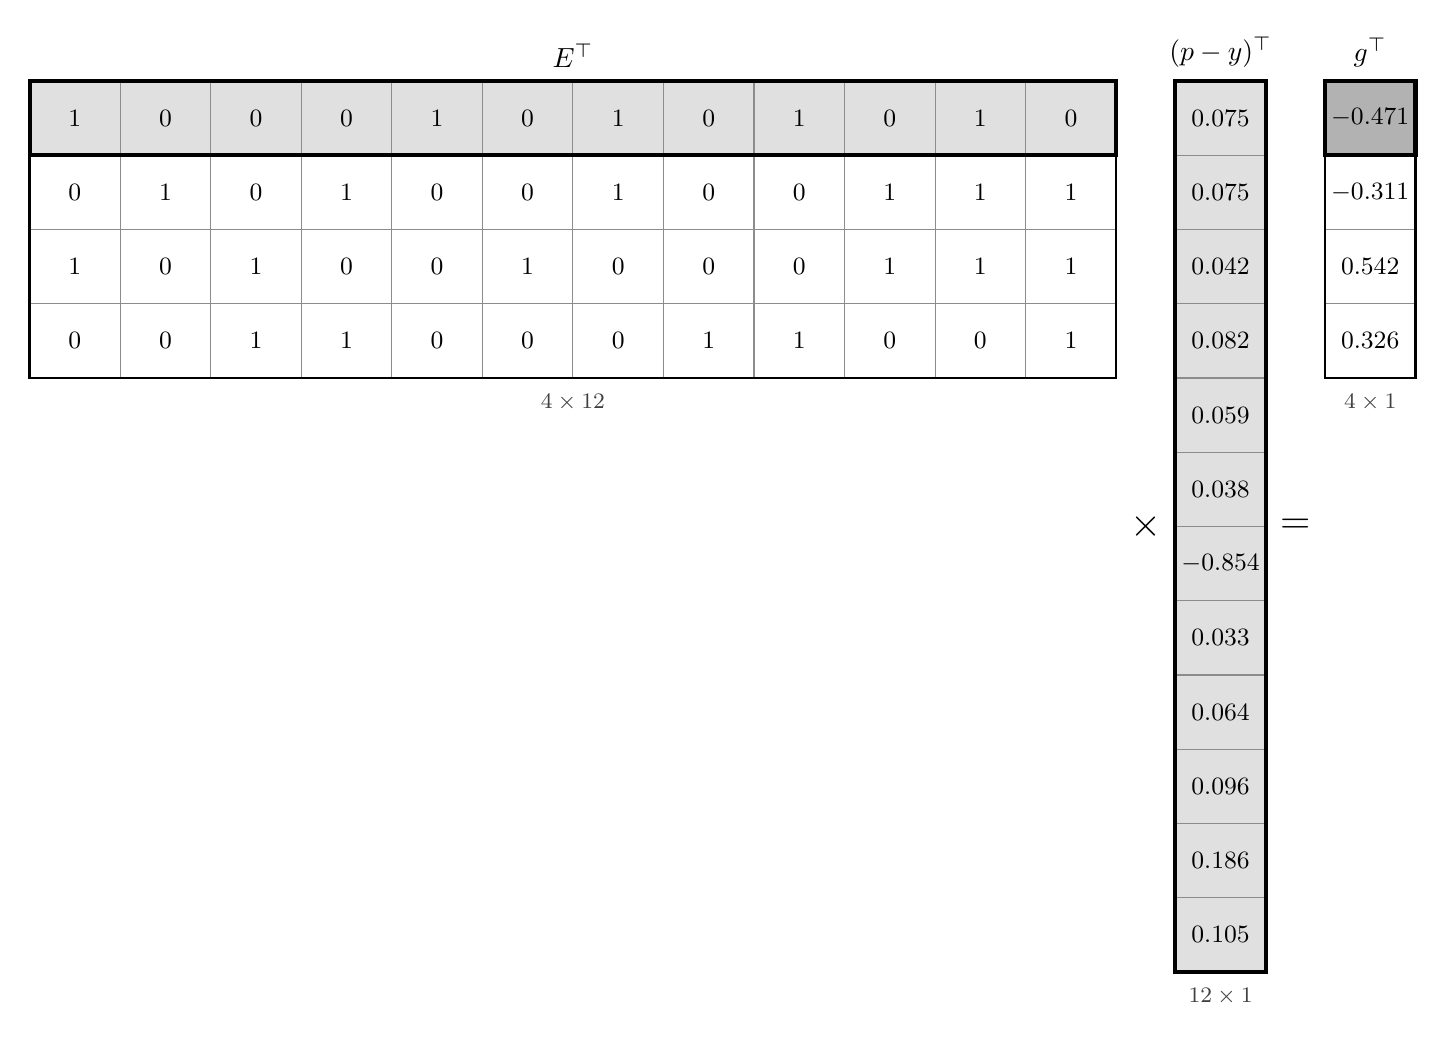
\begin{tikzpicture}
\draw[black!45, fill=black!12] (0.000,0.000) rectangle (1.150,-0.943);
\node[font=\small, text=black] at (0.575,-0.471) {$1$};
\draw[black!45, fill=black!12] (1.150,0.000) rectangle (2.300,-0.943);
\node[font=\small, text=black] at (1.725,-0.471) {$0$};
\draw[black!45, fill=black!12] (2.300,0.000) rectangle (3.450,-0.943);
\node[font=\small, text=black] at (2.875,-0.471) {$0$};
\draw[black!45, fill=black!12] (3.450,0.000) rectangle (4.600,-0.943);
\node[font=\small, text=black] at (4.025,-0.471) {$0$};
\draw[black!45, fill=black!12] (4.600,0.000) rectangle (5.750,-0.943);
\node[font=\small, text=black] at (5.175,-0.471) {$1$};
\draw[black!45, fill=black!12] (5.750,0.000) rectangle (6.900,-0.943);
\node[font=\small, text=black] at (6.325,-0.471) {$0$};
\draw[black!45, fill=black!12] (6.900,0.000) rectangle (8.050,-0.943);
\node[font=\small, text=black] at (7.475,-0.471) {$1$};
\draw[black!45, fill=black!12] (8.050,0.000) rectangle (9.200,-0.943);
\node[font=\small, text=black] at (8.625,-0.471) {$0$};
\draw[black!45, fill=black!12] (9.200,0.000) rectangle (10.350,-0.943);
\node[font=\small, text=black] at (9.775,-0.471) {$1$};
\draw[black!45, fill=black!12] (10.350,0.000) rectangle (11.500,-0.943);
\node[font=\small, text=black] at (10.925,-0.471) {$0$};
\draw[black!45, fill=black!12] (11.500,0.000) rectangle (12.650,-0.943);
\node[font=\small, text=black] at (12.075,-0.471) {$1$};
\draw[black!45, fill=black!12] (12.650,0.000) rectangle (13.800,-0.943);
\node[font=\small, text=black] at (13.225,-0.471) {$0$};
\draw[black!45, fill=white] (0.000,-0.943) rectangle (1.150,-1.886);
\node[font=\small, text=black] at (0.575,-1.414) {$0$};
\draw[black!45, fill=white] (1.150,-0.943) rectangle (2.300,-1.886);
\node[font=\small, text=black] at (1.725,-1.414) {$1$};
\draw[black!45, fill=white] (2.300,-0.943) rectangle (3.450,-1.886);
\node[font=\small, text=black] at (2.875,-1.414) {$0$};
\draw[black!45, fill=white] (3.450,-0.943) rectangle (4.600,-1.886);
\node[font=\small, text=black] at (4.025,-1.414) {$1$};
\draw[black!45, fill=white] (4.600,-0.943) rectangle (5.750,-1.886);
\node[font=\small, text=black] at (5.175,-1.414) {$0$};
\draw[black!45, fill=white] (5.750,-0.943) rectangle (6.900,-1.886);
\node[font=\small, text=black] at (6.325,-1.414) {$0$};
\draw[black!45, fill=white] (6.900,-0.943) rectangle (8.050,-1.886);
\node[font=\small, text=black] at (7.475,-1.414) {$1$};
\draw[black!45, fill=white] (8.050,-0.943) rectangle (9.200,-1.886);
\node[font=\small, text=black] at (8.625,-1.414) {$0$};
\draw[black!45, fill=white] (9.200,-0.943) rectangle (10.350,-1.886);
\node[font=\small, text=black] at (9.775,-1.414) {$0$};
\draw[black!45, fill=white] (10.350,-0.943) rectangle (11.500,-1.886);
\node[font=\small, text=black] at (10.925,-1.414) {$1$};
\draw[black!45, fill=white] (11.500,-0.943) rectangle (12.650,-1.886);
\node[font=\small, text=black] at (12.075,-1.414) {$1$};
\draw[black!45, fill=white] (12.650,-0.943) rectangle (13.800,-1.886);
\node[font=\small, text=black] at (13.225,-1.414) {$1$};
\draw[black!45, fill=white] (0.000,-1.886) rectangle (1.150,-2.829);
\node[font=\small, text=black] at (0.575,-2.357) {$1$};
\draw[black!45, fill=white] (1.150,-1.886) rectangle (2.300,-2.829);
\node[font=\small, text=black] at (1.725,-2.357) {$0$};
\draw[black!45, fill=white] (2.300,-1.886) rectangle (3.450,-2.829);
\node[font=\small, text=black] at (2.875,-2.357) {$1$};
\draw[black!45, fill=white] (3.450,-1.886) rectangle (4.600,-2.829);
\node[font=\small, text=black] at (4.025,-2.357) {$0$};
\draw[black!45, fill=white] (4.600,-1.886) rectangle (5.750,-2.829);
\node[font=\small, text=black] at (5.175,-2.357) {$0$};
\draw[black!45, fill=white] (5.750,-1.886) rectangle (6.900,-2.829);
\node[font=\small, text=black] at (6.325,-2.357) {$1$};
\draw[black!45, fill=white] (6.900,-1.886) rectangle (8.050,-2.829);
\node[font=\small, text=black] at (7.475,-2.357) {$0$};
\draw[black!45, fill=white] (8.050,-1.886) rectangle (9.200,-2.829);
\node[font=\small, text=black] at (8.625,-2.357) {$0$};
\draw[black!45, fill=white] (9.200,-1.886) rectangle (10.350,-2.829);
\node[font=\small, text=black] at (9.775,-2.357) {$0$};
\draw[black!45, fill=white] (10.350,-1.886) rectangle (11.500,-2.829);
\node[font=\small, text=black] at (10.925,-2.357) {$1$};
\draw[black!45, fill=white] (11.500,-1.886) rectangle (12.650,-2.829);
\node[font=\small, text=black] at (12.075,-2.357) {$1$};
\draw[black!45, fill=white] (12.650,-1.886) rectangle (13.800,-2.829);
\node[font=\small, text=black] at (13.225,-2.357) {$1$};
\draw[black!45, fill=white] (0.000,-2.829) rectangle (1.150,-3.772);
\node[font=\small, text=black] at (0.575,-3.300) {$0$};
\draw[black!45, fill=white] (1.150,-2.829) rectangle (2.300,-3.772);
\node[font=\small, text=black] at (1.725,-3.300) {$0$};
\draw[black!45, fill=white] (2.300,-2.829) rectangle (3.450,-3.772);
\node[font=\small, text=black] at (2.875,-3.300) {$1$};
\draw[black!45, fill=white] (3.450,-2.829) rectangle (4.600,-3.772);
\node[font=\small, text=black] at (4.025,-3.300) {$1$};
\draw[black!45, fill=white] (4.600,-2.829) rectangle (5.750,-3.772);
\node[font=\small, text=black] at (5.175,-3.300) {$0$};
\draw[black!45, fill=white] (5.750,-2.829) rectangle (6.900,-3.772);
\node[font=\small, text=black] at (6.325,-3.300) {$0$};
\draw[black!45, fill=white] (6.900,-2.829) rectangle (8.050,-3.772);
\node[font=\small, text=black] at (7.475,-3.300) {$0$};
\draw[black!45, fill=white] (8.050,-2.829) rectangle (9.200,-3.772);
\node[font=\small, text=black] at (8.625,-3.300) {$1$};
\draw[black!45, fill=white] (9.200,-2.829) rectangle (10.350,-3.772);
\node[font=\small, text=black] at (9.775,-3.300) {$1$};
\draw[black!45, fill=white] (10.350,-2.829) rectangle (11.500,-3.772);
\node[font=\small, text=black] at (10.925,-3.300) {$0$};
\draw[black!45, fill=white] (11.500,-2.829) rectangle (12.650,-3.772);
\node[font=\small, text=black] at (12.075,-3.300) {$0$};
\draw[black!45, fill=white] (12.650,-2.829) rectangle (13.800,-3.772);
\node[font=\small, text=black] at (13.225,-3.300) {$1$};
\draw[line width=1.4pt] (0.000,0.000) rectangle (13.800,-0.943);
\draw[line width=0.9pt] (0.000,0.000) rectangle (13.800,-3.772);
\node[anchor=south, font=\normalsize] at (6.900,0.050) {$E^\top$};
\node[anchor=north, font=\footnotesize, text=black!75] at (6.900,-3.852) {$4\times12$};
\draw[black!45, fill=black!12] (14.550,0.000) rectangle (15.700,-0.943);
\node[font=\small, text=black] at (15.125,-0.471) {$0.075$};
\draw[black!45, fill=black!12] (14.550,-0.943) rectangle (15.700,-1.886);
\node[font=\small, text=black] at (15.125,-1.414) {$0.075$};
\draw[black!45, fill=black!12] (14.550,-1.886) rectangle (15.700,-2.829);
\node[font=\small, text=black] at (15.125,-2.357) {$0.042$};
\draw[black!45, fill=black!12] (14.550,-2.829) rectangle (15.700,-3.772);
\node[font=\small, text=black] at (15.125,-3.300) {$0.082$};
\draw[black!45, fill=black!12] (14.550,-3.772) rectangle (15.700,-4.715);
\node[font=\small, text=black] at (15.125,-4.243) {$0.059$};
\draw[black!45, fill=black!12] (14.550,-4.715) rectangle (15.700,-5.658);
\node[font=\small, text=black] at (15.125,-5.186) {$0.038$};
\draw[black!45, fill=black!12] (14.550,-5.658) rectangle (15.700,-6.601);
\node[font=\small, text=black] at (15.125,-6.129) {$-0.854$};
\draw[black!45, fill=black!12] (14.550,-6.601) rectangle (15.700,-7.544);
\node[font=\small, text=black] at (15.125,-7.072) {$0.033$};
\draw[black!45, fill=black!12] (14.550,-7.544) rectangle (15.700,-8.487);
\node[font=\small, text=black] at (15.125,-8.015) {$0.064$};
\draw[black!45, fill=black!12] (14.550,-8.487) rectangle (15.700,-9.430);
\node[font=\small, text=black] at (15.125,-8.958) {$0.096$};
\draw[black!45, fill=black!12] (14.550,-9.430) rectangle (15.700,-10.373);
\node[font=\small, text=black] at (15.125,-9.901) {$0.186$};
\draw[black!45, fill=black!12] (14.550,-10.373) rectangle (15.700,-11.316);
\node[font=\small, text=black] at (15.125,-10.844) {$0.105$};
\draw[line width=1.4pt] (14.550,0.000) rectangle (15.700,-11.316);
\draw[line width=0.9pt] (14.550,0.000) rectangle (15.700,-11.316);
\node[anchor=south, font=\normalsize] at (15.125,0.050) {$(\bm{p}-\bm{y})^\top$};
\node[anchor=north, font=\footnotesize, text=black!75] at (15.125,-11.396) {$12\times1$};
\draw[black!45, fill=black!30] (16.450,0.000) rectangle (17.600,-0.943);
\node[font=\small, text=black] at (17.025,-0.471) {$-0.471$};
\draw[black!45, fill=white] (16.450,-0.943) rectangle (17.600,-1.886);
\node[font=\small, text=black] at (17.025,-1.414) {$-0.311$};
\draw[black!45, fill=white] (16.450,-1.886) rectangle (17.600,-2.829);
\node[font=\small, text=black] at (17.025,-2.357) {$0.542$};
\draw[black!45, fill=white] (16.450,-2.829) rectangle (17.600,-3.772);
\node[font=\small, text=black] at (17.025,-3.300) {$0.326$};
\draw[line width=1.6pt] (16.450,0.000) rectangle (17.600,-0.943);
\draw[line width=0.9pt] (16.450,0.000) rectangle (17.600,-3.772);
\node[anchor=south, font=\normalsize] at (17.025,0.050) {$\bm{g}^\top$};
\node[anchor=north, font=\footnotesize, text=black!75] at (17.025,-3.852) {$4\times1$};
\node[font=\Large] at (14.175,-5.658) {$\times$};
\node[font=\Large] at (16.075,-5.658) {$=$};
\end{tikzpicture}
}\\[2pt]
% AUTO-GENERATED by code/ch*_figs.py -- do not edit
{\small highlighted row (row 1 of $E^\top$) $\cdot$ highlighted column ($\bm{p}-\bm{y}$): $(1)(0.075) + (0)(0.075) + (0)(0.042) + (0)(0.082) + (1)(0.059) + (0)(0.038) + (1)(-0.854) + (0)(0.033) + (1)(0.064) + (0)(0.096) + (1)(0.186) + (0)(0.105) = \mathbf{-0.471}$}
\\[10pt]
\fitR{% AUTO-GENERATED by code/figlib.py helpers -- do not edit
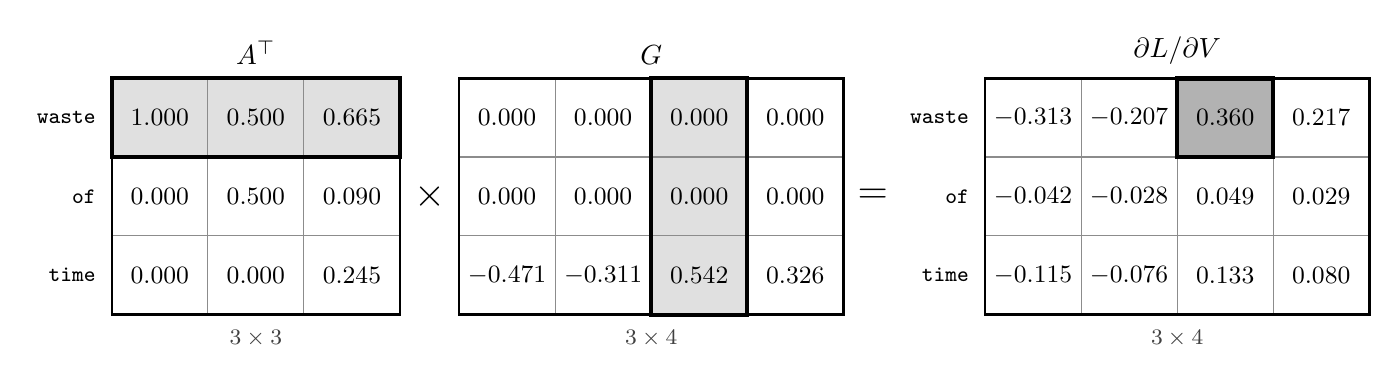
\begin{tikzpicture}
\draw[black!45, fill=black!12] (0.000,0.000) rectangle (1.220,-1.000);
\node[font=\small, text=black] at (0.610,-0.500) {$1.000$};
\draw[black!45, fill=black!12] (1.220,0.000) rectangle (2.440,-1.000);
\node[font=\small, text=black] at (1.830,-0.500) {$0.500$};
\draw[black!45, fill=black!12] (2.440,0.000) rectangle (3.660,-1.000);
\node[font=\small, text=black] at (3.050,-0.500) {$0.665$};
\draw[black!45, fill=white] (0.000,-1.000) rectangle (1.220,-2.001);
\node[font=\small, text=black] at (0.610,-1.501) {$0.000$};
\draw[black!45, fill=white] (1.220,-1.000) rectangle (2.440,-2.001);
\node[font=\small, text=black] at (1.830,-1.501) {$0.500$};
\draw[black!45, fill=white] (2.440,-1.000) rectangle (3.660,-2.001);
\node[font=\small, text=black] at (3.050,-1.501) {$0.090$};
\draw[black!45, fill=white] (0.000,-2.001) rectangle (1.220,-3.001);
\node[font=\small, text=black] at (0.610,-2.501) {$0.000$};
\draw[black!45, fill=white] (1.220,-2.001) rectangle (2.440,-3.001);
\node[font=\small, text=black] at (1.830,-2.501) {$0.000$};
\draw[black!45, fill=white] (2.440,-2.001) rectangle (3.660,-3.001);
\node[font=\small, text=black] at (3.050,-2.501) {$0.245$};
\draw[line width=1.4pt] (0.000,0.000) rectangle (3.660,-1.000);
\draw[line width=0.9pt] (0.000,0.000) rectangle (3.660,-3.001);
\node[anchor=east, font=\footnotesize\ttfamily] at (-0.080,-0.500) {waste};
\node[anchor=east, font=\footnotesize\ttfamily] at (-0.080,-1.501) {of};
\node[anchor=east, font=\footnotesize\ttfamily] at (-0.080,-2.501) {time};
\node[anchor=south, font=\normalsize] at (1.830,0.050) {$A^\top$};
\node[anchor=north, font=\footnotesize, text=black!75] at (1.830,-3.081) {$3\times3$};
\draw[black!45, fill=white] (4.410,0.000) rectangle (5.630,-1.000);
\node[font=\small, text=black] at (5.020,-0.500) {$0.000$};
\draw[black!45, fill=white] (5.630,0.000) rectangle (6.850,-1.000);
\node[font=\small, text=black] at (6.240,-0.500) {$0.000$};
\draw[black!45, fill=black!12] (6.850,0.000) rectangle (8.070,-1.000);
\node[font=\small, text=black] at (7.460,-0.500) {$0.000$};
\draw[black!45, fill=white] (8.070,0.000) rectangle (9.290,-1.000);
\node[font=\small, text=black] at (8.680,-0.500) {$0.000$};
\draw[black!45, fill=white] (4.410,-1.000) rectangle (5.630,-2.001);
\node[font=\small, text=black] at (5.020,-1.501) {$0.000$};
\draw[black!45, fill=white] (5.630,-1.000) rectangle (6.850,-2.001);
\node[font=\small, text=black] at (6.240,-1.501) {$0.000$};
\draw[black!45, fill=black!12] (6.850,-1.000) rectangle (8.070,-2.001);
\node[font=\small, text=black] at (7.460,-1.501) {$0.000$};
\draw[black!45, fill=white] (8.070,-1.000) rectangle (9.290,-2.001);
\node[font=\small, text=black] at (8.680,-1.501) {$0.000$};
\draw[black!45, fill=white] (4.410,-2.001) rectangle (5.630,-3.001);
\node[font=\small, text=black] at (5.020,-2.501) {$-0.471$};
\draw[black!45, fill=white] (5.630,-2.001) rectangle (6.850,-3.001);
\node[font=\small, text=black] at (6.240,-2.501) {$-0.311$};
\draw[black!45, fill=black!12] (6.850,-2.001) rectangle (8.070,-3.001);
\node[font=\small, text=black] at (7.460,-2.501) {$0.542$};
\draw[black!45, fill=white] (8.070,-2.001) rectangle (9.290,-3.001);
\node[font=\small, text=black] at (8.680,-2.501) {$0.326$};
\draw[line width=1.4pt] (6.850,0.000) rectangle (8.070,-3.001);
\draw[line width=0.9pt] (4.410,0.000) rectangle (9.290,-3.001);
\node[anchor=south, font=\normalsize] at (6.850,0.050) {$G$};
\node[anchor=north, font=\footnotesize, text=black!75] at (6.850,-3.081) {$3\times4$};
\draw[black!45, fill=white] (11.090,0.000) rectangle (12.310,-1.000);
\node[font=\small, text=black] at (11.700,-0.500) {$-0.313$};
\draw[black!45, fill=white] (12.310,0.000) rectangle (13.530,-1.000);
\node[font=\small, text=black] at (12.920,-0.500) {$-0.207$};
\draw[black!45, fill=black!30] (13.530,0.000) rectangle (14.750,-1.000);
\node[font=\small, text=black] at (14.140,-0.500) {$0.360$};
\draw[black!45, fill=white] (14.750,0.000) rectangle (15.970,-1.000);
\node[font=\small, text=black] at (15.360,-0.500) {$0.217$};
\draw[black!45, fill=white] (11.090,-1.000) rectangle (12.310,-2.001);
\node[font=\small, text=black] at (11.700,-1.501) {$-0.042$};
\draw[black!45, fill=white] (12.310,-1.000) rectangle (13.530,-2.001);
\node[font=\small, text=black] at (12.920,-1.501) {$-0.028$};
\draw[black!45, fill=white] (13.530,-1.000) rectangle (14.750,-2.001);
\node[font=\small, text=black] at (14.140,-1.501) {$0.049$};
\draw[black!45, fill=white] (14.750,-1.000) rectangle (15.970,-2.001);
\node[font=\small, text=black] at (15.360,-1.501) {$0.029$};
\draw[black!45, fill=white] (11.090,-2.001) rectangle (12.310,-3.001);
\node[font=\small, text=black] at (11.700,-2.501) {$-0.115$};
\draw[black!45, fill=white] (12.310,-2.001) rectangle (13.530,-3.001);
\node[font=\small, text=black] at (12.920,-2.501) {$-0.076$};
\draw[black!45, fill=white] (13.530,-2.001) rectangle (14.750,-3.001);
\node[font=\small, text=black] at (14.140,-2.501) {$0.133$};
\draw[black!45, fill=white] (14.750,-2.001) rectangle (15.970,-3.001);
\node[font=\small, text=black] at (15.360,-2.501) {$0.080$};
\draw[line width=1.6pt] (13.530,0.000) rectangle (14.750,-1.000);
\draw[line width=0.9pt] (11.090,0.000) rectangle (15.970,-3.001);
\node[anchor=east, font=\footnotesize\ttfamily] at (11.010,-0.500) {waste};
\node[anchor=east, font=\footnotesize\ttfamily] at (11.010,-1.501) {of};
\node[anchor=east, font=\footnotesize\ttfamily] at (11.010,-2.501) {time};
\node[anchor=south, font=\normalsize] at (13.530,0.050) {$\partial L/\partial V$};
\node[anchor=north, font=\footnotesize, text=black!75] at (13.530,-3.081) {$3\times4$};
\node[font=\Large] at (4.035,-1.501) {$\times$};
\node[font=\Large] at (9.665,-1.501) {$=$};
\end{tikzpicture}
}\\[2pt]
% AUTO-GENERATED by code/ch*_figs.py -- do not edit
{\small highlighted row (\texttt{waste}'s column of $A$) $\cdot$ highlighted column (column 3 of $G$): $(1.000)(0.000) + (0.500)(0.000) + (0.665)(0.542) = \mathbf{0.360}$}

\captionof{figure}{Two steps of the backward pass with the toy's real numbers. Top: $E^\top$ (one column per word, in
vocabulary order) times $(\bm{p}-\bm{y})^\top$ gives $\bm{g}$, the gradient reaching \tok{time}'s attention
output (shown standing up).
Bottom: $A^\top G$ gives the gradient of every value arrow. Row \tok{waste} is the biggest because \tok{time}
gave \tok{waste} the biggest share in the forward pass: whoever was listened to most gets corrected most.
Our script checks the resulting $\partial L/\partial W_V = X^\top(\partial L/\partial V)$ against probing all 16
numbers.}
\end{minipage}\par\medskip

We checked every row of the table on the toy of Chapter 3, with a random $G$, against probing each of the 48
numbers in $W_Q$, $W_K$, $W_V$: relative errors $\nAppAErrQ$, $\nAppAErrK$ and $\nAppAErrV$.

\begin{checkq}
Why is it $A^\top G$ and not $AG$ or $GA$?
\begin{options}
\item $AG$ is also correct; the order does not matter.
\item The result must have the shape of $V$ ($T\times d_k$), and $A^\top G$ is the only product of these two
that does, while summing over the right index.
\item Transposes always appear in the backward pass.
\end{options}
\end{checkq}

\subsection*{A.5\quad Through a residual connection}

Chapter 5 adds each block's output to its input: $\bm{y}=\bm{x}+f(\bm{x})$ (He and colleagues, 2016). By
the chain rule,
\[
\frac{\partial L}{\partial \bm{x}} = \frac{\partial L}{\partial \bm{y}} + \frac{\partial L}{\partial
\bm{y}}\,J_f ,
\]
where $J_f$ is the table of slopes of $f$. The first term passes the gradient back \emph{untouched}. Without
the ``$\bm{x}+$'', the gradient is multiplied by a $J_f$ at every layer, and Chapter 1's fading memory
returns: we stacked layers of $\tanh(\bm{h}W)$ with small random weights and measured the size of the
gradient that reaches the input.

\begin{center}
\small
\begin{tabular}{@{}l c c@{}}
\toprule
layers & without residual & with residual\\
\midrule
10 & $\nAppAPlainTen$ & \nAppAResidTen\\
50 & $\nAppAPlainFifty$ & \nAppAResidFifty\\
\bottomrule
\end{tabular}
\end{center}
Without the residual path, after 50 layers essentially nothing reaches the first layer, so it cannot learn.
With it, the signal arrives intact. Probing check on a 5-layer residual stack: $\nAppAErrResid$.

\Summary{the gradient through attention follows from the chain rule and the shape rule, saturation and
masking both show up as zeros in it, and a residual connection gives the gradient a path that is never
multiplied away.}

\begin{lookingback}
\begin{enumerate}[label=(\arabic*),leftmargin=1.6em]
\item (Chapter 3) The transpose in $QK^\top$ arranges keys as columns. Where does a transpose reappear in
the backward pass, and what does the shape rule say about it?
\item (Chapter 1) Which break of the RNN does the residual table above echo?
\end{enumerate}
\end{lookingback}

\subsection*{Exercises}
\begin{exercise}
Find the slope of $y=x^3$ at $x=2$, first by the rise-over-run of a tiny step, then by expanding $(2+h)^3$.
\end{exercise}
\begin{exercise}
Probabilities over three words are $(0.7, 0.2, 0.1)$ and the right word is the second. Write the slope of
the loss on each of the three scores. Which score goes up after a downhill step?
\end{exercise}
\begin{exercise}
For a sentence of $T=5$ tokens, what are the shapes of $\partial L/\partial S$ and $\partial L/\partial W_K$
when $d=8$ and $d_k=4$?
\end{exercise}
\begin{exercise}
Explain in one sentence, using A.4, why a token never gets a gradient from a later token's score.
\end{exercise}

\subsection*{Answers to Appendix A}

\paragraph{Check yourself A.1.} (b). The extra is exactly $h$: $(6h+h^2)/h=6+h$. It is not rounding (a), and
the derivative is $2x=6$ (c).
\paragraph{Check yourself A.2.} (b). $p_y=1$ gives $p_y-1=0$. (a) would push further towards a word that
already has all the probability.
\paragraph{Check yourself A.3.} (b). The shape rule decides. (a) is false: $AG$ sums over the wrong index.
(c) is false in general: many backward steps have no transpose.

\paragraph{Exercise A.1.} $(2+h)^3 = 8+12h+6h^2+h^3$, so the rise-over-run is $12+6h+h^2\to12$. Probing
gives \nAppAExCube.
\paragraph{Exercise A.2.} $\bm{p}-\bm{y}=\nAppAExCE$. Only the second slope is negative, so only the second
score goes up.
\paragraph{Exercise A.3.} $\partial L/\partial S$ has the shape of $S$, $5\times5$; $\partial
L/\partial W_K$ has the shape of $W_K$, $8\times4$.
\paragraph{Exercise A.4.} Masked cells have $A_{ij}=0$, and the formula for $\partial L/\partial S_{ij}$ is
multiplied by $A_{ij}$, so it is zero there.
